\chapter{Website Construction}

As mentioned earlier, I chose to build my Character Comparison Tool as a website for the following reasons:
    * Many historians are not computer savvy, so an interface they are already familiar with may feel more natural to them.
    * Relieves the burden of having to download, install, configure, and debug experimental software.
    * Accessible to anyone who uses the internet.
    * Provide  a platform to which many people can use and contribute to.
    
    \begin{figure}{}
    \parbox{12cm}{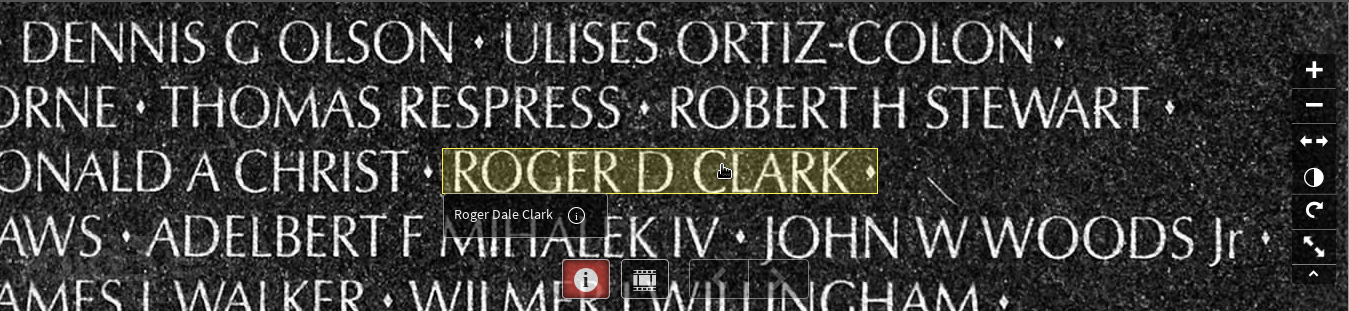
\includegraphics[width=12cm]{fold3.png}}
    \caption{Vietnam Memorial page at fold3.com}
    \label{Vietnam Memorial inspiration}
    \end{figure}
    
    My website needed to have to ability to browse between works, 
    
        My Website overview:
            My website is fairly typical and includes the following:
                Front-End:  jQuery based user-interface
                Back-End:   Django, Gunicorn, and Nginx with a PostgreSQL database
                
            When the user is browsing an individual page he / she sees a calligraphy page, inside a re-sizable window.
                Green boxes are overlay-ed on top of all characters in this page that map to the Character Database.
                
                The page is naturally navigable with a zoom in/out bar and drag-able window.
                Every-time the page is dragged or the zoom level is changed, all character boxes are adjusted so they stay precisely the same position and size with respect to the parent page.
                
                As the user mouses over a character, it's box turns blue indicating it is a candidate for selection.
                
                Once a character is selected a slider, it's box turns red. A slider at the bottom of the screen becomes populated with characters which are attributed to that same author
                
                When any character in the slider is clicked it opens up a new browser window showing the parent page.  (I really think an Ajax thing where we load the new image into a side-by-side window would be much better)
                
                This allows another researcher to (hopefully) easily and (also hopefully) comprehensively compare a large number of similar, but different characters, in order to discern the subtle differences between and among Calligraphic works
                
                
                    My results:
        *  I created a website that permits browsing uploaded images of calligraphy texts.
            +Bounding boxes are overlay-ed on top of characters on the 
                *These bounding boxes follow characters during navigation (Zoom and drag)
                *Zooming is continuous, not discrete, this way researchers can see the two characters side-by-side for a more effective comparison
            +To the best of my knowledge, this is the first application to allow easy and direct navigation between similar characters on scanned high resolution, continuously zoom-able images.
